\documentclass[conference]{IEEEtran} 
\IEEEoverridecommandlockouts
% The preceding line is only needed to identify funding in the first footnote. If that is unneeded, please comment it out.
\usepackage{cite}
\usepackage{amsmath,amssymb,amsfonts}
\usepackage{algorithmic}
\usepackage{graphicx}
\usepackage{textcomp}
\usepackage{xcolor}
\usepackage{array}
\usepackage{multirow}
\def\BibTeX{{\rm B\kern-.05em{\sc i\kern-.025em b}\kern-.08em
    T\kern-.1667em\lower.7ex\hbox{E}\kern-.125emX}}
\begin{document}

\title{An In-Depth Analysis of Student Prompts Using CharlieBot \\
{\footnotesize \textsuperscript{*}Note: Sub-titles are not captured in Xplore and
should not be used}
\thanks{Identify applicable funding agency here. If none, delete this.}
}

\author{\IEEEauthorblockN{1\textsuperscript{st} Rodrigo Prestes Machado}
\IEEEauthorblockA{\textit{dept. Informática} \\
\textit{Instituto Federal do Rio Grande do Sul}\\
Porto Alegre, Brazil \\
0000-0003-0428-6387}
\and
\IEEEauthorblockN{2\textsuperscript{nd} Given Name Surname}
\IEEEauthorblockA{\textit{dept. name of organization (of Aff.)} \\
\textit{name of organization (of Aff.)}\\
City, Country \\
email address or ORCID}
\and
\IEEEauthorblockN{3\textsuperscript{rd} Given Name Surname}
\IEEEauthorblockA{\textit{dept. name of organization (of Aff.)} \\
\textit{name of organization (of Aff.)}\\
City, Country \\
email address or ORCID}
\and
\IEEEauthorblockN{4\textsuperscript{th} Given Name Surname}
\IEEEauthorblockA{\textit{dept. name of organization (of Aff.)} \\
\textit{name of organization (of Aff.)}\\
City, Country \\
email address or ORCID}
\and
\IEEEauthorblockN{5\textsuperscript{th} Given Name Surname}
\IEEEauthorblockA{\textit{dept. name of organization (of Aff.)} \\
\textit{name of organization (of Aff.)}\\
City, Country \\
email address or ORCID}
\and
\IEEEauthorblockN{6\textsuperscript{th} Given Name Surname}
\IEEEauthorblockA{\textit{dept. name of organization (of Aff.)} \\
\textit{name of organization (of Aff.)}\\
City, Country \\
email address or ORCID}
}

\maketitle

\begin{abstract}
This document is a model and instructions for \LaTeX.
This and the IEEEtran.cls file define the components of your paper [title, text, heads, etc.]. *CRITICAL: Do Not Use Symbols, Special Characters, Footnotes, 
or Math in Paper Title or Abstract.
\end{abstract}

\begin{IEEEkeywords}
component, formatting, style, styling, insert
\end{IEEEkeywords}

\section{Introduction}

%What is the problem to be solved?

% Are there any existing solutions?

% Which is the best?

% What is its main limitation?

% What do you hope to achieve?

\section{Background}

\begin{table*}[htbp]
\caption{Categories and Descriptions}
    \begin{center}
    \begin{tabular}{|p{3cm}|p{3cm}|p{5cm}|}
    \hline
    \textbf{Critical Thinking} & \textbf{Category} & \textbf{Description} \\
    \hline
    \multirow{6}{3cm}{Tends to promote} & Debugging Help & Prompts that seek
    help to identify, fix errors, or understand the provided code snippet. \\
    & Conceptual Questions & Prompts that are more about understanding concepts
    or algorithms rather than specific code. \\
    & Student Correction & Prompts where the student corrects the bot. \\
    \hline
    \multirow{6}{3cm}{Tends not to promote} & Code Snippet & Prompts that ask
    for a specific part of the code, like a function or a segment. \\
    & Complete Solution & Prompts that request an entire solution or a complete
    code snippet. \\
    & Multiple Question Exercise & Prompts where the user wants to solve a
    multiple-question exercise. \\
    \hline
    \multirow{3}{3cm}{Neutral} & Language Change & Prompts that request a change
    of idiom. \\
    & Uncategorized & Prompts that do not fit into any of the above categories. \\
    \hline
    \end{tabular}
    \label{tab:categories}
    \end{center}
\end{table*}

\section{Method}

Initially, we identified four initial categories were identified for classifying
student messages with the bot, as outlined in the article "Coding with AI: How
Are Tools Like ChatGPT Being Used by Students in Foundational Programming
Courses." These initial categories are as follows: (1) Debugging Help: Messages
that seek assistance in identifying and fixing errors or understanding the
provided code snippet; (2) Code Snippet: Messages requesting a specific part
of the code, such as a function or a segment; (3) Conceptual Questions: Messages
focused on understanding concepts or algorithms rather than specific code;
and (4) Complete Solution: Messages requesting an entire solution or a complete
code snippet.
\\
Upon further exploration of the data, it was determined that four additional
categories could be added, resulting in a total of eight categories: (1)
Multiple Question Exercise: Messages where the user seeks to solve a multiple-question
exercise; (2) Student Correction: Messages where the student corrects the bot;
(3) Language Change: Messages requesting a change of language; and (4)
Uncategorized: Messages that do not fit into any of the aforementioned
categories.
\\
Subsequently, these eight categories were input into Claude.ai, accompanied by
detailed instructions on the desired structure of the input and the expected
format of the output. For each conversation in the CharlieBot log, a .csv file
was downloaded, and Claude was tasked with classifying the user messages into
one of the eight categories.

The classifications made by Claude were then manually reviewed. In cases where
there was disagreement with the classification, manual adjustments were made,
and the accuracy of Claude's classification was recorded. Each conversation
with CharlieBot was saved into a .csv file containing the original conversation,
along with two additional columns: "Classification" to denote the category and
"AI" to indicate Claude's accuracy.

As new categorizations were completed, an example was submitted to Claude's
knowledge base to enhance accuracy. Initially, Claude began with an example
representing 1\% of the total memory of its knowledge base. As classifications
were progressively completed, more examples were provided to Claude to increase
the percentage of its knowledge base occupied by relevant examples.

Upon completion of all categorizations, all resulting .csv files were consolidated
for final counts and analysis using the Pandas library. This methodology
facilitated an efficient categorization of student messages, thereby enabling
a comprehensive analysis of how tools such as ChatGPT are utilized in foundational
programming courses.

\section{Result and Discussion}

Bellow is the distribution of the messages in the categories:

\centerline{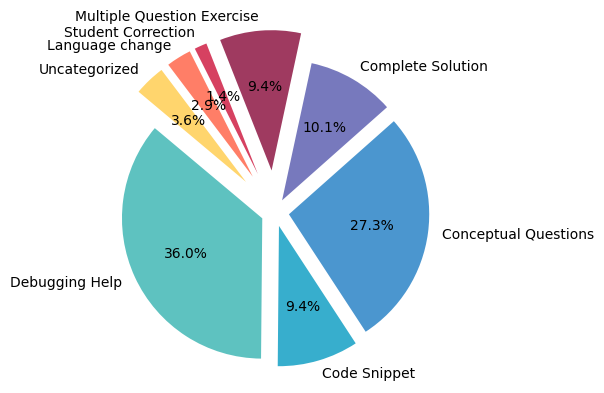
\includegraphics[scale=0.6]{figures/figure1.png}}

Approximately 64\% of the messages pertain to categories associated with
critical thinking, corroborating with the findings of
\cite{10.1007/978-3-031-64299-9_20}. In contrast, around 28\% of the messages
indicate a preference among students for ready-made answers.



\section{Conclusion}

\bibliographystyle{IEEEtran}
\bibliography{references}

\vspace{12pt}
\color{red}
IEEE conference templates contain guidance text for composing and formatting conference papers. Please ensure that all template text is removed from your conference paper prior to submission to the conference. Failure to remove the template text from your paper may result in your paper not being published.

\end{document}
